\documentclass[paper=a4paper,jafontsize=9pt,head_space=15mm,gutter=20mm,
twocolumn,number_of_lines=49, line_length=26zw]{myuarticle}

\begin{document}

\title{{\LARGE\bfseries\gtfamily 環境情報のセンシングを用いた他者の環境評価を表現するロボットシステム}}
\author{\\\ 22120165 中村龍造 \\ (指導教員 : 佐藤宏樹)\\ \\}
\date{}
\maketitle

\section{まえがき}
私たちの周りには、人間以外にも多くの存在が共存している。それらの存在は、それぞれ独自の感覚や基準で環境を捉えているが、私たちはその感覚を直接共有することができない。このような「他者」の経験を理解し、共感することは、多様な存在との共生を考える上で重要な課題となっている。

本システムでは、取得した環境データに対して、人間、動植物、非生物などといった複数の主体からの評価基準を設定し、評価結果をロボットの身体的動作を通して表現する。本システムを通じて、ユーザーが「他者」にとっての快適さを知り、「他者」への理解、関心を深めることで、多様な存在との対話の機会創出を目指す。

\section{関連研究と課題}

環境センシング分野では,IoTやセンサー技術の発展により,室内環境の継続的なモニタリングが可能となっており\cite{Saini-2020-IndoorAirQualityMonitoring},個々人の主観による評価も必要とされている\cite{Coulby-2020-ScopingReviewTechnologicalApproaches}.

「他者」視点の表現に関する取り組みとして,Marshmallow Laser Feastの「In the Eyes of the Animal」\cite{Dezeen-2015-MarshmallowLaserFeastsEyes}やソンのrapoptosis\cite{--ソンヨン}がある.前者は動物の視覚体験を,後者は非生物の視点を表現している.また,Human Robot Interactionの分野では,Breazeal\cite{C.Breazeal-2004-SocialInteractionsHRIRobot}が人間と協働するパートナーとしてのロボットのあり方を提示している.

以上から本研究では,人間,動植物,非生物など,様々な「他者」を基準に,それらから見た環境の快・不快を,ロボットの身体的動作で表現するシステムを開発する.

\section{システム要件}
本システムの開発にあたって,次の3点を要件とする.
\begin{itemize}
  \item ロボット:自身が代弁する「他者」の特徴が動きに現れている
  \item 評価システム:「他者」基準の評価が適切に行われる
  \item 全体:ユーザー自身とそれ以外との環境の受け取り方の違いを体験することができる
\end{itemize}

\subsection{全体のフロー}
システム全体は,ユーザー,環境,センサー,ロボット,本システムの5つの間で動作する.システム全体のフローを図\ref{fig:system-flow}に示す.

\fboxsep=0pt            %画像と枠線をくっつける.
\fboxrule=1pt            %枠線の太さを1ptにする.
\begin{figure}[h]
  \centering
  \fbox{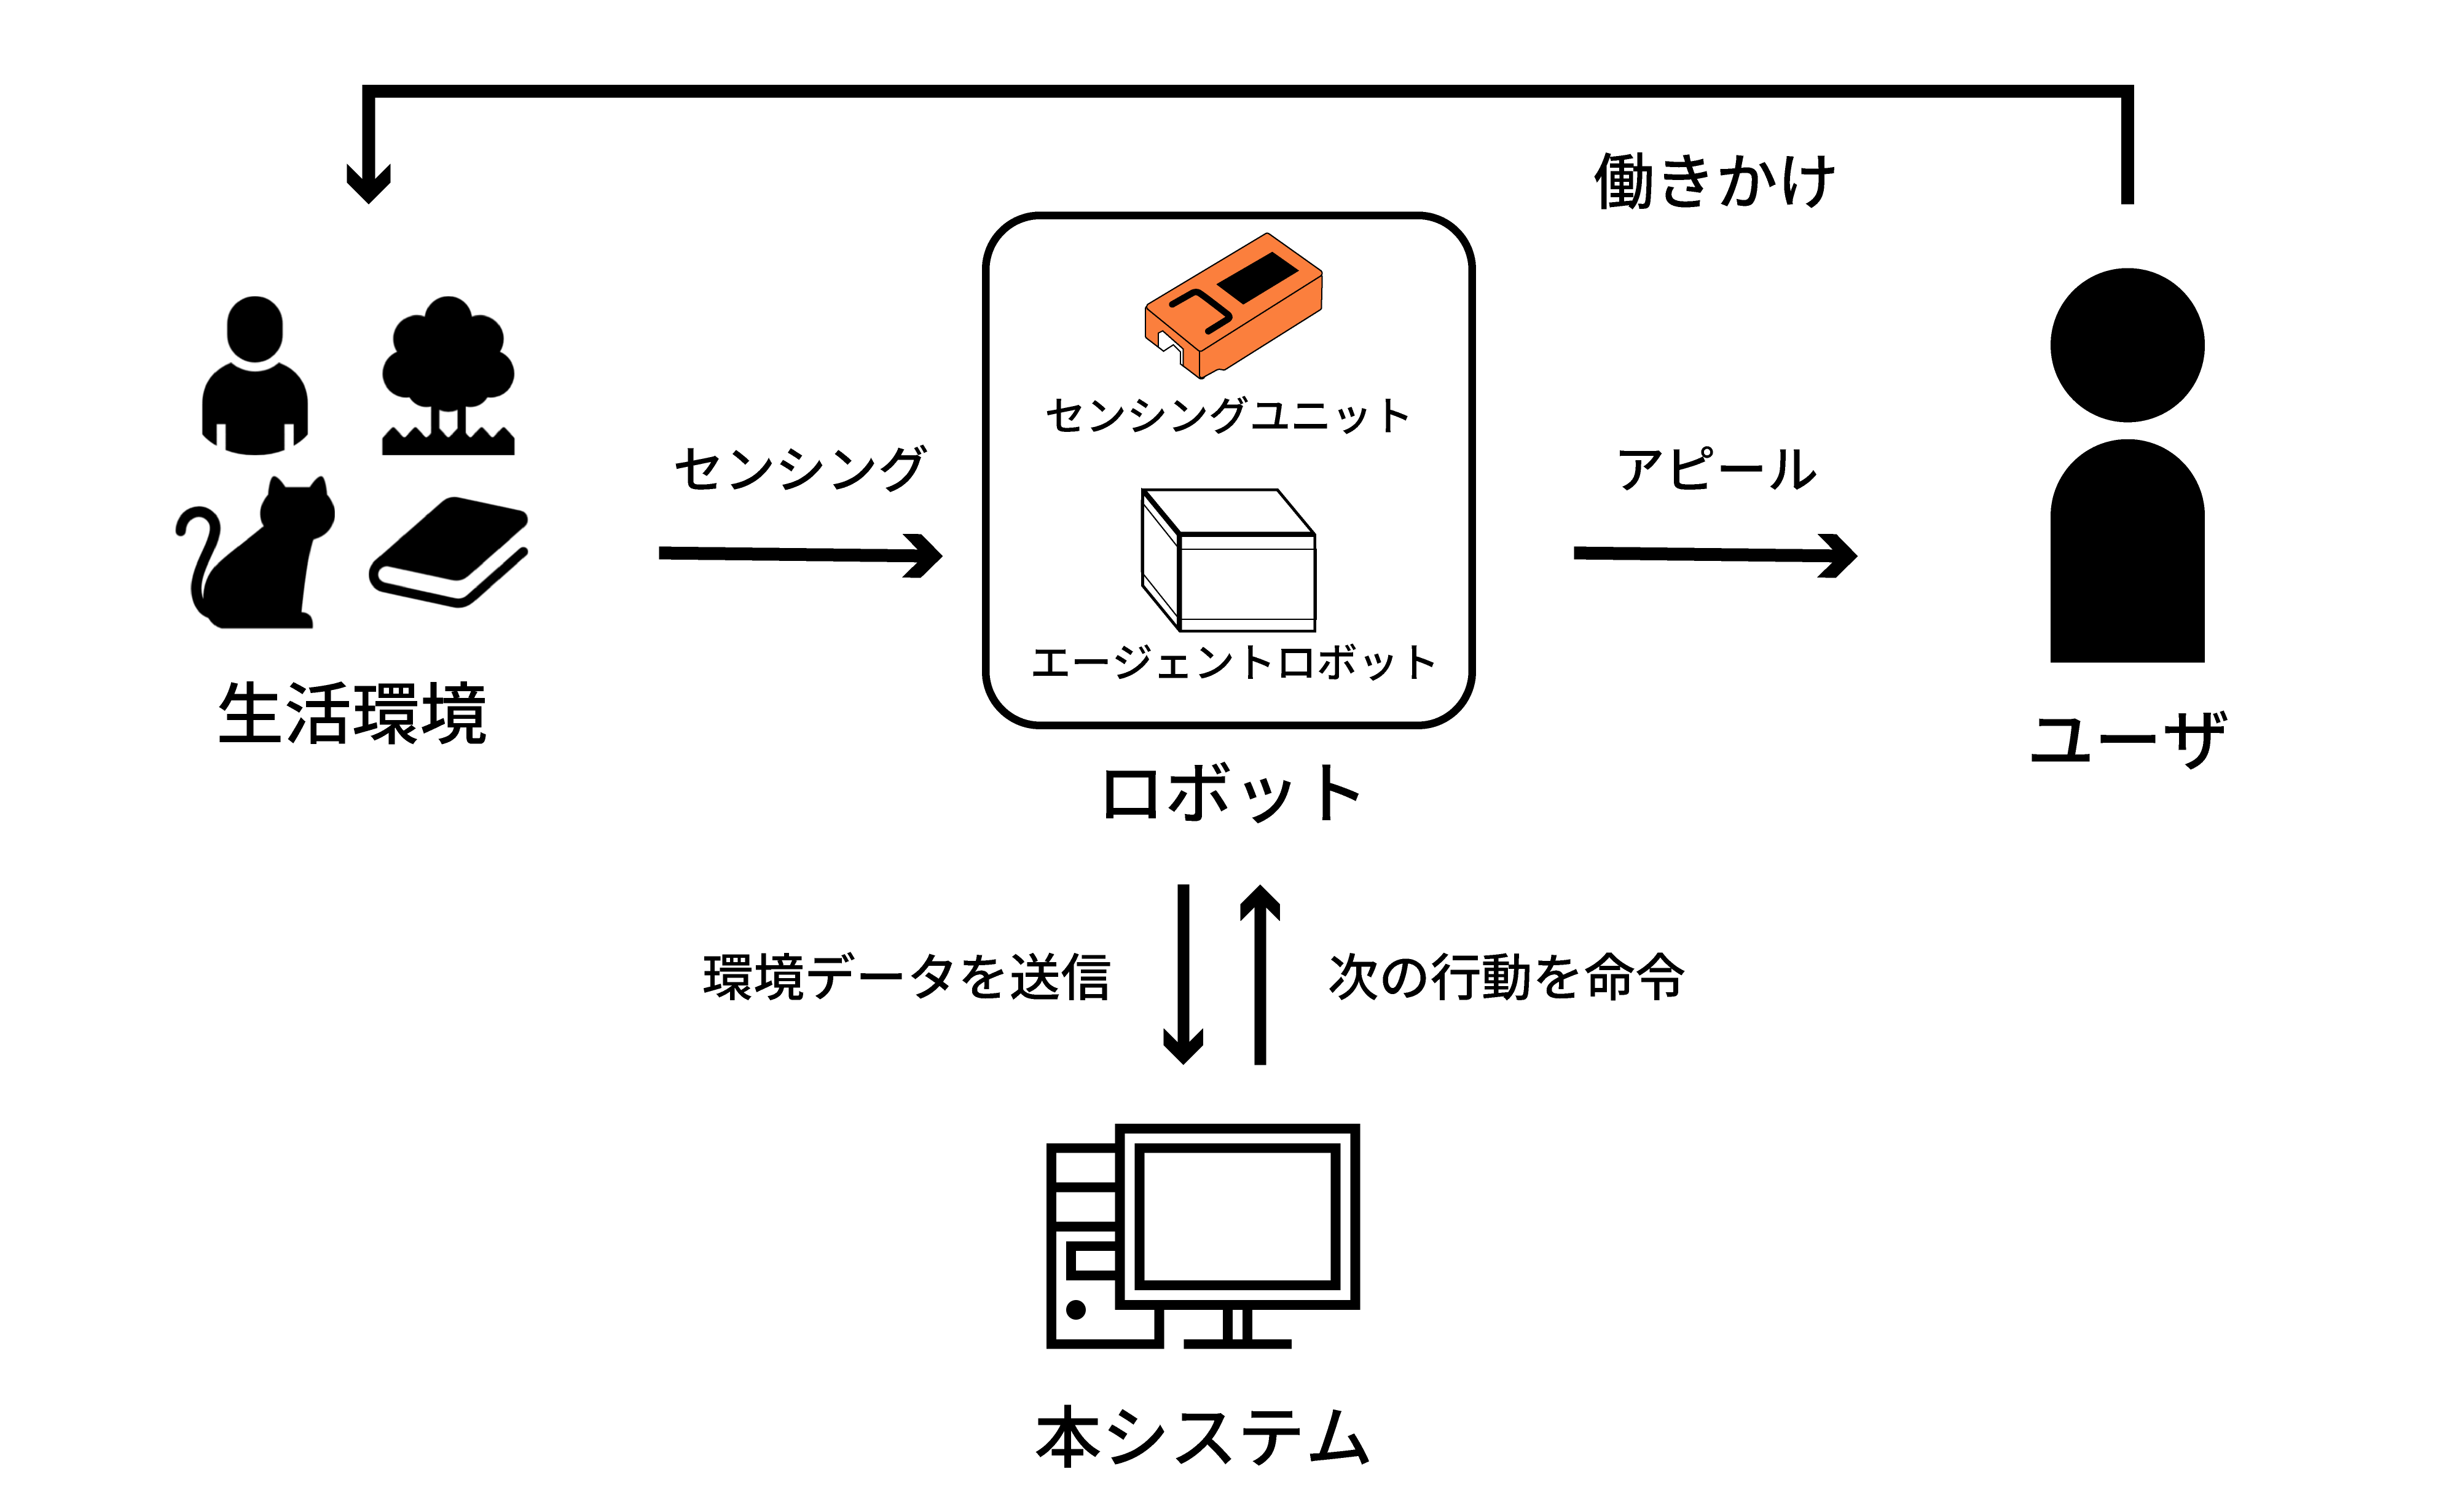
\includegraphics[keepaspectratio, clip,
  width=0.8\columnwidth]{resources/system_flow.png}}
  \caption{システム全体のフロー図}
  \label{fig:system-flow}
\end{figure}

はじめに本システムが,センサーを通じて生活空間の環境データを取得する.「他者」を基準とした評価,評価に応じて快・不快をアピールするなどの行動命令を現実空間のロボットに送信する.ロボットは行動命令に従って人間にアピールする.それを見た人間が環境や「他者」に対して働きかけることで,他者にとってより快適な環境を得るシステムとなっている.

\section{本システムの実装}
本システムは,センシングシステム,評価システム,アクション生成システム,ロボット制御システムから構成される.ハードウェアは,センシングデバイスにM5StickC(M5Stack社)を,ロボットにtoio(SONY社)を選定した.本システムの構造を図\ref{fig:system-structure}に示す.

\fboxsep=0pt            %画像と枠線をくっつける.
\fboxrule=1pt            %枠線の太さを1ptにする.
\begin{figure}[h]
  \centering
  \fbox{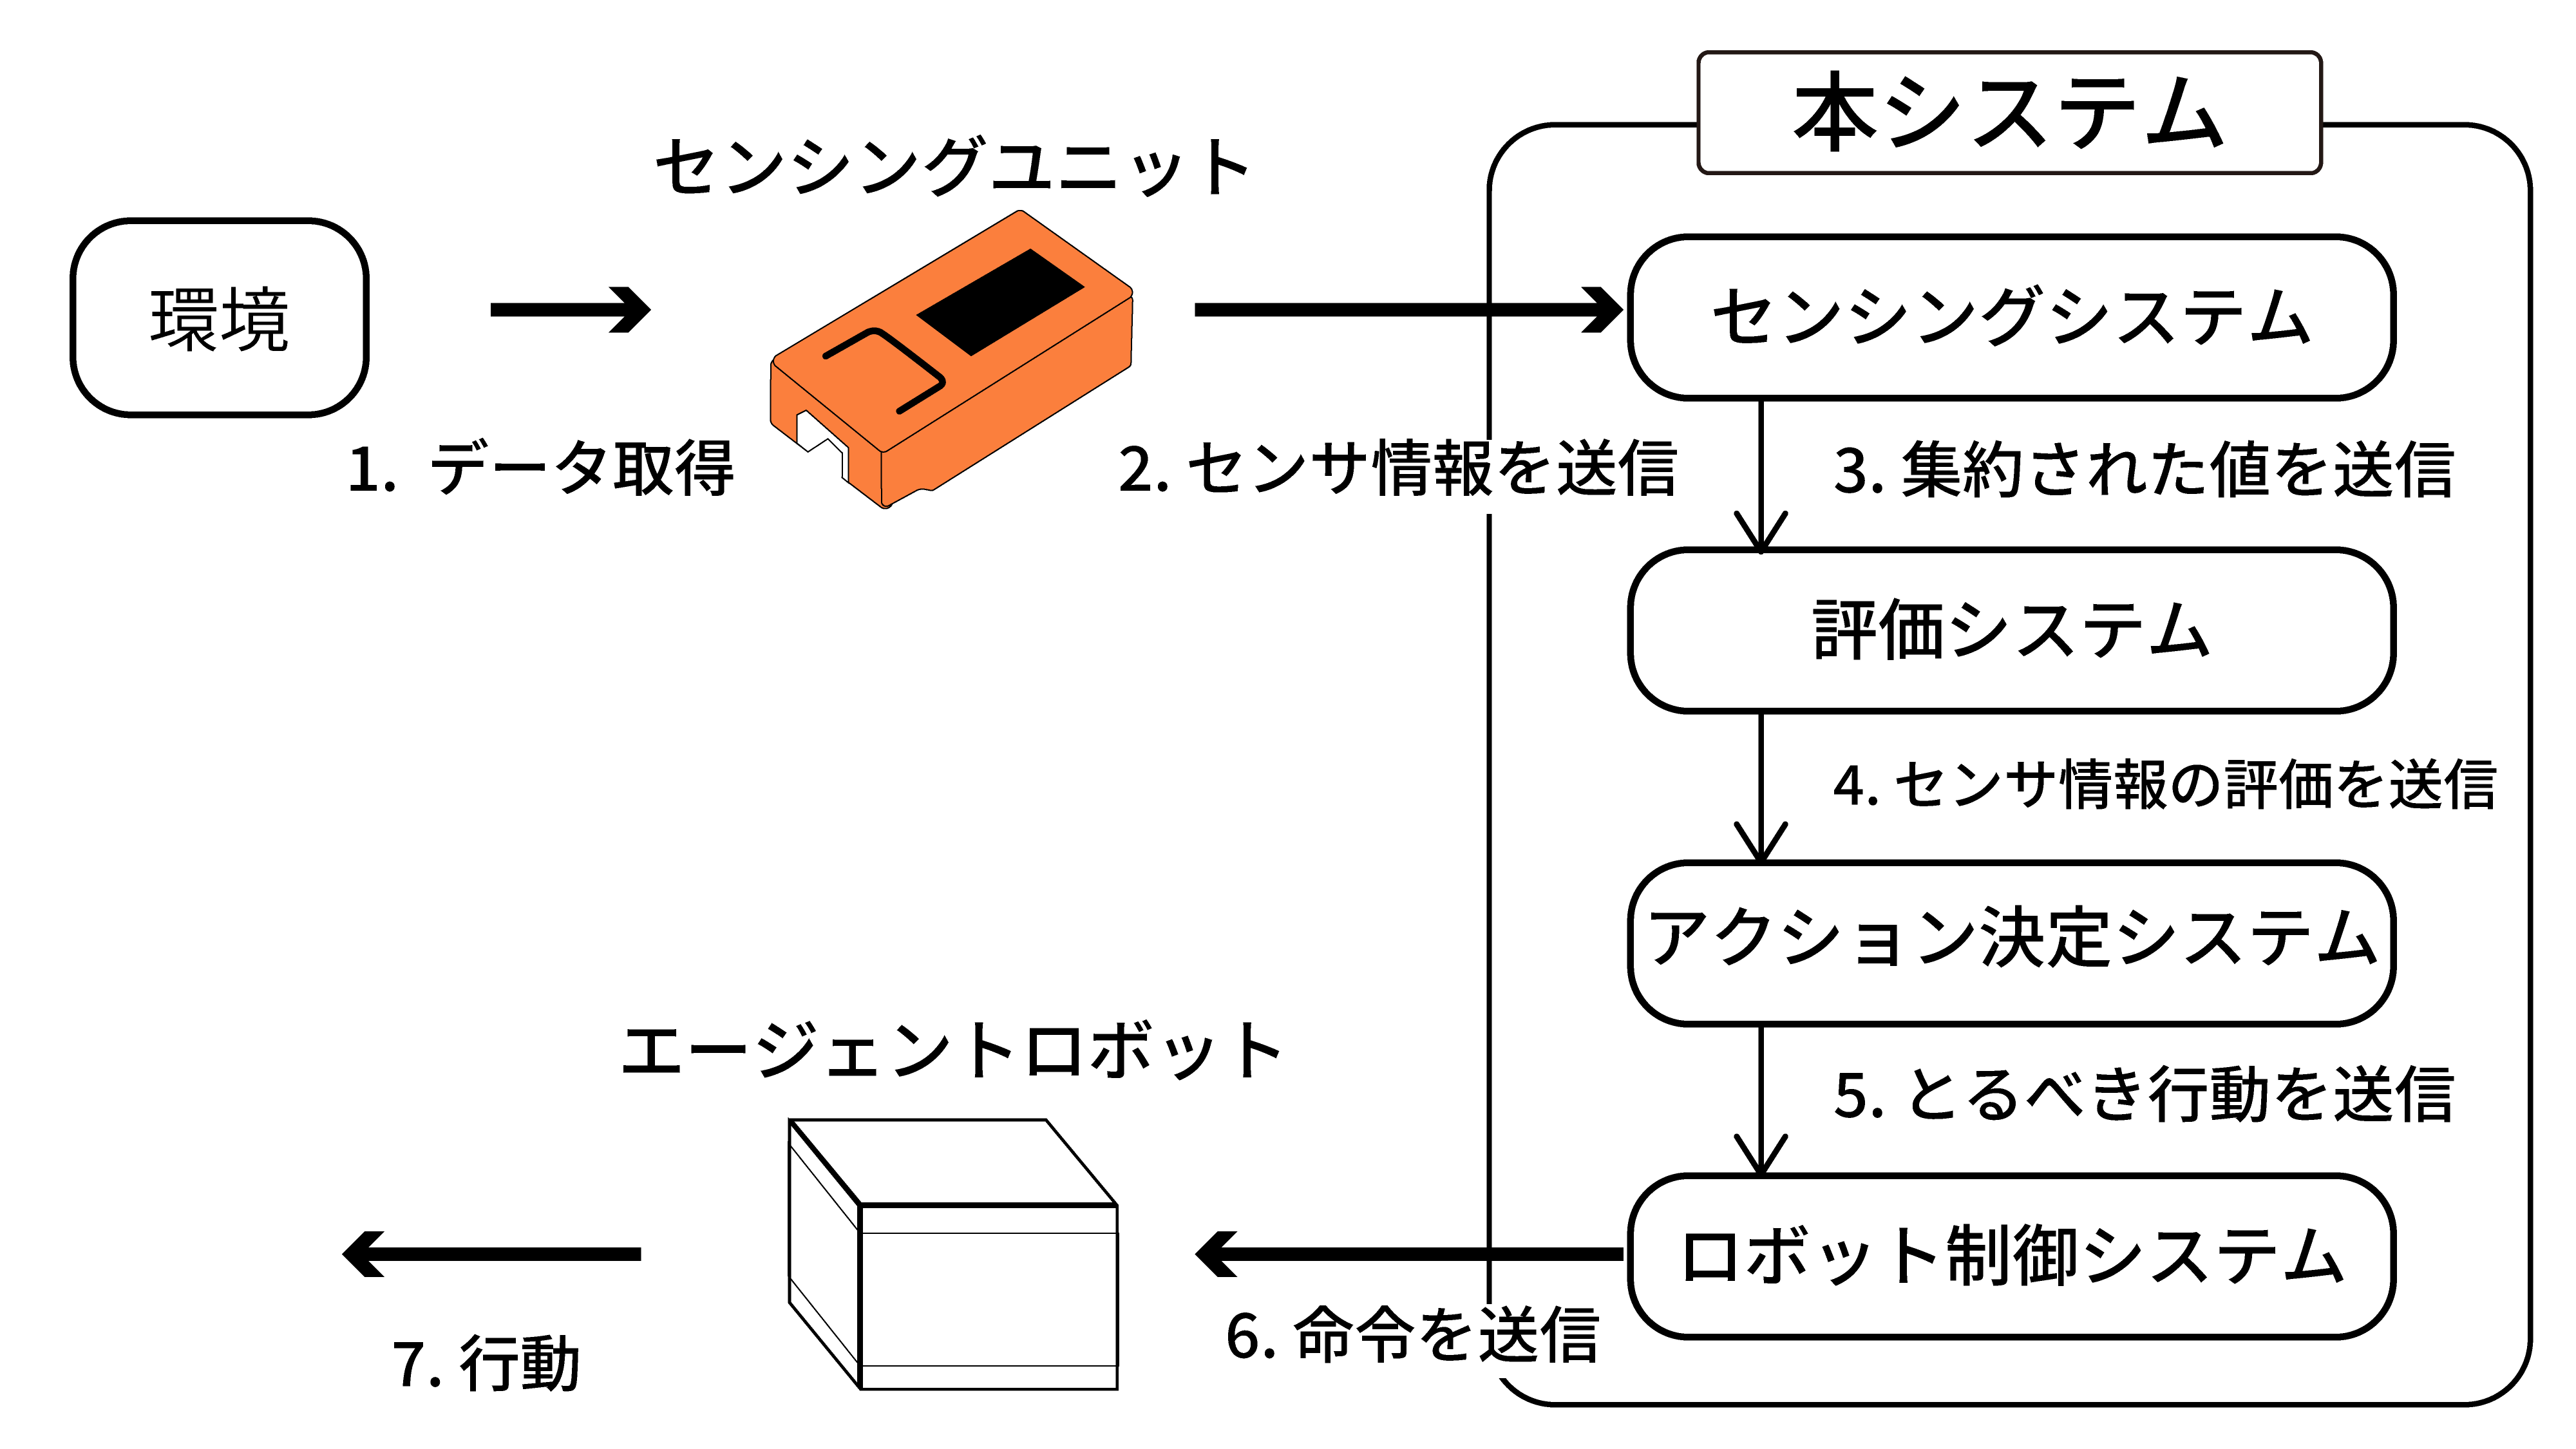
\includegraphics[keepaspectratio, clip,
  width=0.8\columnwidth]{resources/system_structure.png}}
  \caption{本システムの構造図}
  \label{fig:system-structure}
\end{figure}

\subsection{センシングシステム}

センシングシステムは,センサ側とクライアント側の2つの部分から構成される.センサ側では環境データの取得と,シリアル通信での送信を行う.

\subsection{評価システム}
評価システムでは,センサーシステムから環境データを取得・評価し,評価データを返す.評価システムは主体とその評価対象ごとに作成する.評価データは,環境データと評価基準値との差をスコアとして所持しており.対象データの評価では,例えば人間に適した気温であれば24-18℃などと,あらかじめ対象データの最適範囲を設定する.現在の気温が最適範囲から外れた場合,上回れば正の,下回れば負のスコアをもたせる.アクション生成システムではスコアをもとに生成するアクションを決定する.

\subsection{アクション生成システム}
アクション生成システムでは,評価システムから取得した評価データをもとに評価に応じたアクション命令をロボット制御システムへ送る.送信するアクションは主体および対象の環境データごとに事前に作成しておく必要がある.サンプルとしてデザインしたアクションには,岡田ら\cite{岡田-2017-弱いロボ}の「弱いロボット」の「よたよた」とした動きを取り入れることで,効果的にユーザーに働きかけることを狙った.

アクションは「コマンド」のキューで構成される.コマンドはロボット動作用のより低レベルな命令と,動作の所要時間を所持しており,一連のコマンドを実行することで,1つの意味あるアクションを表現する.

\subsection{ロボット制御システム}
ロボット制御システムでは,実機toioとシステム上のtoioを識別するためのデータ管理および,アクション生成システムから取得したアクションの実行を行う.

\section{本システムの制約}

提案にあたって,本システムの制約について述べる.

エージェントは,本システムとの通信が可能な範囲に配置する必要がある.今回はBluetooth通信を使用しているため,物理的な仕切りなどによって通信が不安定になりやすい.またエージェントの動作がユーザーから認識できる場所にある必要がある.想定しているエージェントの動作環境は屋内であり,屋外の生活環境での使用は考えられていない.

表現の面では,ロボットが持つモジュールによって可能なアクションが異なる.また本システムが対象とできる「他者」は,評価基準が明確で,評価データがセンサーによって取得可能なものに限られる.同時に制御できるロボットの数にも制限があるため,大量の他者を同時に表現することは難しい.

\section{今後の展望}
本システムの展望として,アクションデザインでは,ロボットどうしの協調やより効果的な動作のデザイン検討が考えられる.センシング面では,快・不快をより正確に表現するデータの検討や,キャリブレーションの追加等が可能である.また異なるセンサ,ロボットを使用することで,新しいユーザー体験を生み出すことが期待される.

\section{あとがき}
本研究では,環境データを「他者」の視点から評価し,ロボットの身体的動作を通じて表現するシステムを開発した.M5StickCとtoioを用いたプロトタイプシステムの実装により,「他者」にとっての快・不快を直感的に理解できるインタフェースを実現した.特に,『弱いロボット』の概念を取り入れることで,ユーザーを自然にシステムフローに組み込むことができた.

今後は,より多様な「他者」の表現や,ロボット同士の協調動作の実装など,システムの拡張を進めていく.

%  ----- 参考文献 -----
% 参考文献リストの「参考文献」のスタイル
\renewcommand{\refname}{ 参考文献}
\bibliography{ref}
\bibliographystyle{junsrt}
\end{document}
